
%%%%%% 

\section{LessLinux as thinclient}

Since autumn 2012 LessLinux includes programs and scripts to run as a thinclient with minimal overhead. This targets primarily environments where LessLinux is booted via the network and converted to a thinclient OS with just a few boot parameters. For now the functionality to comfortably access \index{RDP} RDP logins is implemented, audio redirection works good if optional parameters are specified (chooser only). Access to printers, local USB drives and other local USB devices is work in progress.

\subsection{Booting to Remmina}

\begin{figure}[htbp]
\center{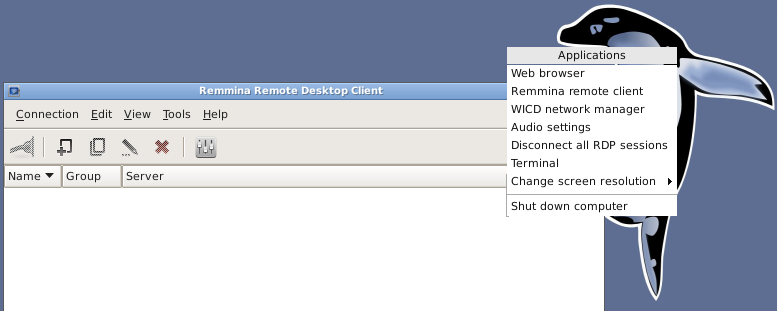
\includegraphics[width=12cm]{admin/remmina.png}}
\caption{\label{fig:remmina} Just specifying \texttt{xinitrc=/etc/lesslinux/xinitrc\_remote} will open Remmina on an otherwise empty desktop. Right click on the desktop background to get a menu with some useful programs (also available when booting to chooser or RDP login mask).}
\end{figure}

If you just pass the parameters 

\begin{verbatim}
xinitrc=/etc/lesslinux/xinitrc_remote
\end{verbatim} 

you will end up in an empty desktop with a \index{Remmina} Remmina window open. Remmina allows for access to RDP, VNC, reverse VNC and SSH servers. Since all settings are lost upon reboot, this option is primarily interestinng for admins who want to be able to remotely login to servers from any machine in the network that boots via PXE.

With the \texttt{xinitrc\_remote}
the default window manager is OpenBox. Right click on the desktop to get a simple menu from where you can start Firefox, a terminal window or the mixer (for remote audio). 

\subsection{Booting to an RDP login mask}

\begin{figure}[htbp]
\center{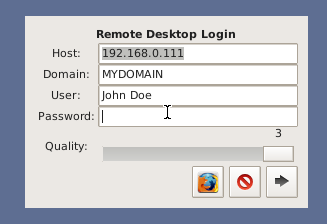
\includegraphics[width=8cm]{admin/rdpmask.png}}
\caption{\label{fig:rdpmask} The RDP login mask is configured via boot command line and does not need a separate configuration file.}
\end{figure}

The easiest way is booting to a simple login mask: To enable thinclient mode specify

\begin{verbatim}
xinitrc=/etc/lesslinux/xinitrc_remote
\end{verbatim} 
 
and additionally to enter the RDP login mask

\begin{verbatim}
rdesktop=|12.34.56.78|username|domain|2|
\end{verbatim} 

Those parameters are IP address of the RDP server, user name and domain name (optional). The user name might be encoded as in HTTP URIs: \texttt{Kemal\%20Atat\%C3\%BCrk} is unescaped to \texttt{Kemal Atat�rk} - however due to character set limitiations you should try to avoid umlauts in user names. The optional integer specifies the quality of the connection: 0 is low quality, but fast, 3 is highest quality, but slower. Use 0 for very slow connections (modem, 3G), 1 in broadband connections (or 3.5G, 4G), 2 (default) in typically congested ethernets and 3 for very fast ethernets with low congestion. Those numerical values map to the following parameters upon execution of \texttt{xfreerdp}

\begin{itemize}
\item \textbf{0} \texttt{-x m -a 16}  - 16 bit color depth, modem experience
\item \textbf{1} \texttt{-x b -a 16}  - 16 bit color depth, broadband experience
\item \textbf{2} \texttt{-x l -a  32} - 32 bit color depth, LAN experience
\item \textbf{3} \texttt{-x 180 -a  32} - 32 bit color depth, LAN experience plus font smoothing and Desktop Composition
\end{itemize}

RDP Sessions start in full screen. You might toggle full screen with \texttt{Ctrl+Alt+Enter}, e.g. to access the local OpenBox menu or start a local Firefox instance.

\subsection{Booting to a chooser}

\begin{figure}[htbp]
\center{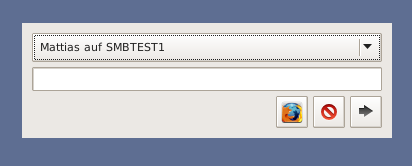
\includegraphics[width=8cm]{admin/chooser.png}}
\caption{\label{fig:chooser} The chooser is configured by an XML file that is loaded from the boot medium or via the network.}
\end{figure}

More comfort and more flexibility is provided by the optional chooser. To use it, you have to prepare an XML file with one block per entry. This XML file has to be accessible via FTP, HTTP or TFTP. Currently only RDP connections are available via chooser, \index{VNC} VNC, Nomachine NX, XDMCP and Citrix \index{ICA} ICA will follow eventually. Add the parameters 

\begin{verbatim}
xinitrc=/etc/lesslinux/xinitrc_remote
\end{verbatim} 
 
and

\begin{verbatim}
chooser=tftp://server/path/chooser.xml 
\end{verbatim} 

to boot into chooser mode. If you are booting from a USB drive, you can put the \texttt{chooser.xml} on the boot partition (usually the second partition on the thumb drive) and specify 

\begin{verbatim}
chooser=file:///lesslinux/boot/chooser.xml 
\end{verbatim}

Alternatively when remastering a CD with \texttt{chooser.xml} in the root directory of the ISO 9660 file system, specify 

\begin{verbatim}
chooser=file:///lesslinux/cdrom/chooser.xml 
\end{verbatim}

In both cases make sure to specify \texttt{toram=0} to prevent LessLinux from unmounting \texttt{/lesslinux/boot} or \texttt{/lesslinux/cdrom} before the chooser.xml there can be used.

A sample XML file \texttt{chooser.xml} could look like:

\begin{verbatim}
<chooser>
  <connect nicename="John Doe" host="192.168.0.23" 
           proto="rdp" user="john" domain="MYDOMAIN">
    <default inet="192.168.0.17" />
    <default ether="00:24:8c:6b:5d:e4" />
    <param>-x l -a 32</param>
  </connect>
  <connect nicename="Jane Doe" host="192.168.0.23" 
           proto="rdp" user="jane" domain="MYDOMAIN">
    <default inet="192.168.0.18" />
    <param>-x 180 -a 32</param>
    <param>--plugin rdpsnd --data tsmf:audio:alsa:plughw:0,0 --</param>
  </connect>
  <connect nicename="Alice X" host="192.168.0.24" 
           proto="rdp" user="alice" domain="OTHERDOMAIN">
    <default inet="192.168.0.19" />
    <param>-x l -a 32</param>
  </connect>
  <connect nicename="Admininstrator on Server 1" host="192.168.0.23" 
           proto="rdp" user="Administrator" />
  <connect nicename="Admininstrator on Server 2" 
           host="192.168.0.24" proto="rdp" user="Administrator" />
</chooser>
\end{verbatim}

The first to entries specifiy connections to the RDP server \texttt{192.168.0.23}, with the domain \texttt{MYDOMAIN}. The parameters specify LAN experience for John Doe and remote audio as well as font smoothing and compositing for Jane Doe. The \texttt{default} tag specifies on which client machines an entry is selected as default. On the client machines with local MAC adress  \texttt{00:24:8c:6b:5d:e4} or local IP \texttt{192.168.0.17} John Doe will be shown as default, on \texttt{192.168.0.18} Jane Doe will be shown as default. Feel free to play with parameters for \texttt{xfreerdp} to get the best performance according to your network's latency, bandwidth and congestion.

\subsection{Using XDMCP}

The X Display Manager Control Protocol \index{XDMCP} that is used in several unix only environments is work in progress and not yet reflected in any cheatcodes. It will become available soon with the sole limitation that the keymap of the initially started X server will be US english. Depending on your Display Manager some special character in passwords won't be at the used keys. As soon as you are logged in most desktop environments take care for setting the user's keyboard layout.

\subsection{Local printers}

\begin{figure}[htbp]
\center{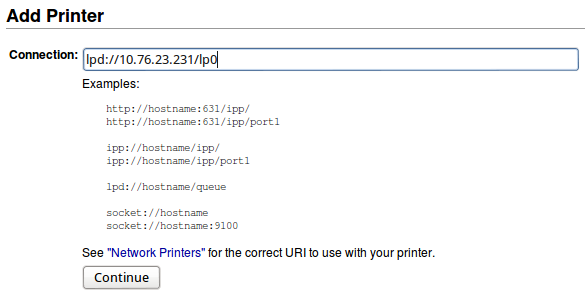
\includegraphics[width=12cm]{admin/printer.png}}
\caption{\label{fig:printers} Local USB printers can easily be shared: This screenshot shows adding USB printer \texttt{/dev/usb/lp0} on LessLinux host 10.76.23.231 to a CUPS server that centralizes spooling.}
\end{figure}

Minimal support for local printers is now provided with BusyBox' LPD. This is considered experimental, it might work or not, and parameters will change in the future without further notice. Specify 

\begin{verbatim}
printers=|lp0|lp1|
\end{verbatim} 

to enable printing to the USB printers available at \texttt{/dev/usb/lp0} and \texttt{/dev/usb/lp1}. This will start a line printer daemon with queues having the same names as the printers \texttt{lp0} and \texttt{lp1}. Since no filtering is done, the clients printing have to send raw output in a format the printer understands.



